\documentclass[border=0.5cm]{standalone}
\usepackage{calculator}
\usepackage{tikz}
\usetikzlibrary{arrows, arrows.meta, positioning}

\tikzset{    
    disk/.style={ thick },
    traj/.style={ thin, dotted, -Latex },
    point/.style={ color=black, circle, scale=0.3, fill },
    partition/.style={ right, scale=0.75 },
    label/.style={ scale=0.5, black, below = 0.5mm }
}

\definecolor{light-gray}{gray}{0.45}

\def\xMin{0}
\def\xMax{3}
\def\yMin{0}
\def\yMax{3}
\def\xWidth{1}
\def\oPacity{0.75}
\def\ySlant{0.5}
\def\xSlant{-0.9}
\def\z{50}
\def\speed{0.1}
\def\R{0.05}

\newcommand{\drawFrame}[5]{
    \fill[#5, opacity=0.15] (#1*\xWidth,#2*\xWidth) rectangle (#3*\xWidth,#4*\xWidth);
    \draw[#5, dashed] (#1*\xWidth+\speed,#2*\xWidth+\speed) rectangle (#3*\xWidth-\speed,#4*\xWidth-\speed);
    \draw[#5] (#1*\xWidth,#2*\xWidth) rectangle (#3*\xWidth,#4*\xWidth);
}
\newcommand{\drawGrid}{
    \fill[white,fill opacity=\oPacity] (\xMin,\yMin) rectangle (\xMax,\yMax);
    \draw[step=\xWidth, very thin, light-gray] (\xMin,\yMin) grid (\xMax,\yMax);
}
\newcommand{\drawFlocks}[1]{
    \draw [fill=lime   ](A#1) circle (\R) ;
    \draw [fill=magenta](B#1) circle (\R) ;
    \draw [fill=teal   ](C#1) circle (\R);
}
\newcommand{\drawLabels}[1]{
    \node[label] at (A#1) {$a$};
    \node[label] at (B#1) {$b$};
    \node[label] at (C#1) {$c$};
}
\newcommand{\drawTrajs}[1]{
        \def\i{}
        \ADD{#1}{-1}{\i}
        \draw[traj] (A\i) -- (A#1);
        \draw[traj] (B\i) -- (B#1);
        \draw[traj] (C\i) -- (C#1);
}

\begin{document}
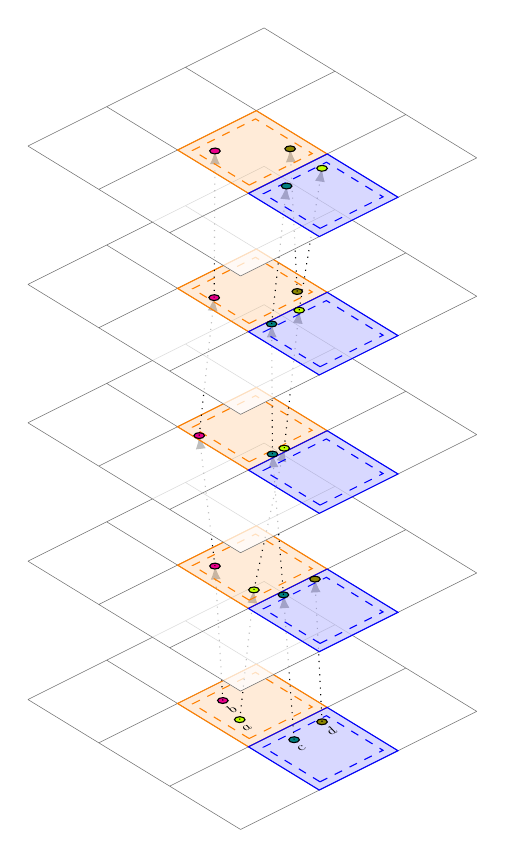
\begin{tikzpicture}
    \begin{scope}
        [yshift=0*\z, every node/.append style={yslant=\ySlant,xslant=\xSlant},yslant=\ySlant,xslant=\xSlant]
        \coordinate (A0) at (1.25, 1.40);
        \coordinate (B0) at (1.35, 1.75);
        \coordinate (C0) at (1.40, 0.80);
        \coordinate (D0) at (1.80, 0.85);

        \drawGrid
        \drawFrame{1}{1}{2}{2}{orange};
        \drawFrame{1}{0}{2}{1}{blue};
        \drawFlocks{0}
        \drawLabels{0}
        \draw[fill=olive](D0) circle (\R);
        \node[label] at (D0) {$d$};
    \end{scope}
    	
    \begin{scope}
        [yshift=1*\z, every node/.append style={yslant=\ySlant,xslant=\xSlant},yslant=\ySlant,xslant=\xSlant]
        \coordinate (A1) at (1.25, 1.20);
        \coordinate (B1) at (1.25, 1.75);
        \coordinate (C1) at (1.40, 0.95);
        \coordinate (D1) at (1.80, 0.95);

        \drawTrajs{1}
        \draw[traj] (D0) -- (D1);
        \drawGrid
        \drawFrame{1}{1}{2}{2}{orange};
        \drawFrame{1}{0}{2}{1}{blue};
        \drawFlocks{1}
        \draw[fill=olive](D1) circle (\R);
    \end{scope}
    
    \begin{scope}
        [yshift=2*\z, every node/.append style={yslant=\ySlant,xslant=\xSlant},yslant=\ySlant,xslant=\xSlant]
        \coordinate (A2) at (1.50, 1.05);
        \coordinate (B2) at (1.05, 1.75);
        \coordinate (C2) at (1.35, 1.05);

        \drawTrajs{2}
        \drawGrid
        \drawFrame{1}{1}{2}{2}{orange};
        \drawFrame{1}{0}{2}{1}{blue};
        \drawFlocks{2}
    \end{scope}

    \begin{scope}
        [yshift=3*\z, every node/.append style={yslant=\ySlant,xslant=\xSlant},yslant=\ySlant,xslant=\xSlant]
        \coordinate (A3) at (1.60, 0.95);
        \coordinate (B3) at (1.15, 1.65);
        \coordinate (C3) at (1.25, 0.95);
        \coordinate (D3) at (1.80, 1.20);

        \drawTrajs{3}
        \drawGrid
        \drawFrame{1}{1}{2}{2}{orange};
        \drawFrame{1}{0}{2}{1}{blue};
        \drawFlocks{3}
        \draw[fill=olive](D3) circle (\R);
    \end{scope}
    
    \begin{scope}
        [yshift=4*\z, every node/.append style={yslant=\ySlant,xslant=\xSlant},yslant=\ySlant,xslant=\xSlant]
        \coordinate (A4) at (1.80, 0.85);
        \coordinate (B4) at (1.25, 1.75);
        \coordinate (C4) at (1.35, 0.85);
        \coordinate (D4) at (1.80, 1.30);

        \drawTrajs{4}
        \draw[traj] (D3) -- (D4);
        \drawGrid
        \drawFrame{1}{1}{2}{2}{orange};
        \drawFrame{1}{0}{2}{1}{blue};
        \drawFlocks{4}
        \draw[fill=olive](D4) circle (\R);
    \end{scope}
\end{tikzpicture}
\end{document} 
